\documentclass{report}
\usepackage{nips13submit_e,times}
\usepackage[utf8x]{inputenc}
\usepackage{amsfonts}
\usepackage{indentfirst}
\usepackage{hyperref}
\usepackage{graphicx}
\usepackage{enumerate}
\usepackage{amsmath}
\usepackage{subfigure} 
\usepackage{amsopn}
\title{Project-II by group TORONTO}
\author{Michalina Pacholska \And Jakub Sygnowski}
\addtolength{\voffset}{-1.25cm}
\addtolength{\textheight}{+1.5cm}
\addtolength{\hoffset}{-2cm}
\addtolength{\textwidth}{+4cm}
\nipsfinalcopy
\newcommand{\mychapter}[2]{
    \setcounter{chapter}{#1}
    \setcounter{section}{0}
    \chapter*{#2}
}
\begin{document}
\maketitle
\begin{abstract}
This report describes our work on second project done for Machine Learning class at EPFL in Fall 2014. We were given...
\end{abstract}
\begingroup
\renewcommand{\cleardoublepage}{}
\renewcommand{\clearpage}{}
\mychapter{1}{Music recommendation system}
\endgroup
\section{Problem and dataset descriptions}
During the project, we were first given a train dataset, which we should analyse and learn our algorithms on, and then, a week before the deadline, we were given a test dataset, for which we should give our predictions. In the train dataset, there is information about $A=15082$ artists and $U=1774$ users. Dataset consists of three matrices:
\begin{itemize}
    \item $1\times A$ vector of artists' names - we did not use that.
    \item $U \times A$ matrix of listen count of each artist by every user. This matrix is called $Ytrain$.
    \item $U \times U$ matrix of social network between users. This matrix is caled $Gtrain$.
\end{itemize}

Both $Ytrain$ and $Gtrain$ are sparse. Social matrix includes $22904$ ones, which denoted the social connection between users. This mean that our users have on average $12.9109$ friends. $Gtrain$ is symmetric and binary.

In case of listen counts, zero in the matrix meant that the user did not heard of given artist and didn't listen to him, but not necessarily didn't like him. There is $69617$ non-zero entries in the matrix, which constitute $0.26\%$ of it. Our problem is to predict for some given (user, artist) pairs what the listen counts would be if user would have been heard about this artist before.

The test data consists of three matrices as well:
\begin{itemize}
\item $Ytest_{weak\_pairs}$ of size $1774\times 15082$ - binary matrix denoting which (user, artist) pair should we predict. $u$-th row of this matrix corresponds to the user described by the $u$-th row of $Ytrain$ and $Gtrain$
\item $Gstrong$ of size $93 \times 1867 = 1774 + 93$ - binary matrix representing social connections of $93$ new users added to our network. We are supposed to predict their listen counts based only on their social information. Submatrix of last $93$ columns of $Gstrong$ is symmetric.
\item $Ytest_{strong\_pairs}$ of size $93 \times 15082$ representing which (user, artist) pairs should we predict for the newly added users.
\end{itemize}

Our predictions will be graded based on true values, which course teacher has. Let our answer be $predicted$ and real value would be $real$, then error associated with our prediction is meant to be $log(predicted) - log(real)$. Then the teacher will calculate mean squared error \cite{mse} of our prediction using different artist and user types and grade us based on the results (and this raport).

\section{Train data analysis and preparation}
We took a look at various distributions of the data and we have found out that:
\begin{enumerate}[1.]
\item Most of the artists have only few distinct listeners. (\ref{fig:artistListeners}). First, we have $1262$ artists for which there don't exist even a single listener, so we cannot predict anything reasonable for them. Then, $90.26\%$ of all the artists have at most $5$ different listeners.
\item Distribution of all listen counts (for all artists and all users) is not Gaussian: \ref{fig:listenCounts}. It rather resembles $\frac{1}{x}$ or $e^{-x}$. We tried applying various transformations to normalize the data. We decided to use logarithm, which gave us effect shown on \ref{fig:logListenCounts}.
\end{enumerate}
\begin{figure}[!h]
\center
\subfigure[For each (user, artist) listen count value - how many times does it occur in $Y_{train}$ ]{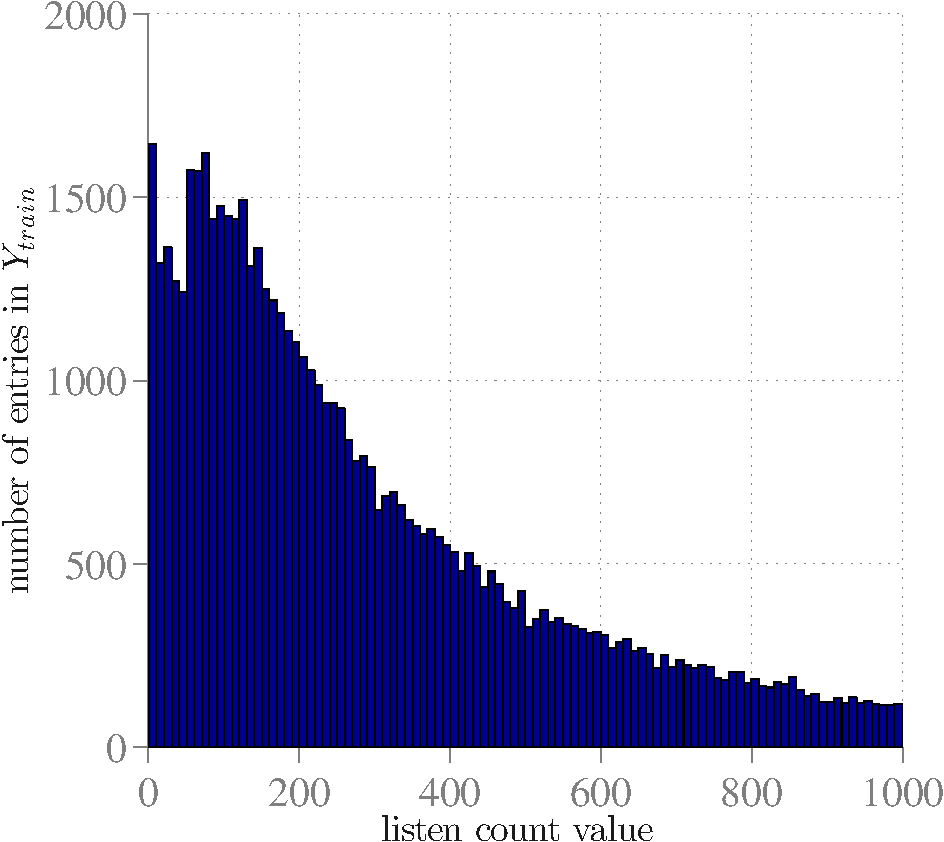
\includegraphics[width=2.5in]{../figures/listen_counts-crop.pdf} \label{fig:listenCounts}}
\subfigure[Same histogram as in \ref{fig:listenCounts}, but after taking logarithm of each value]{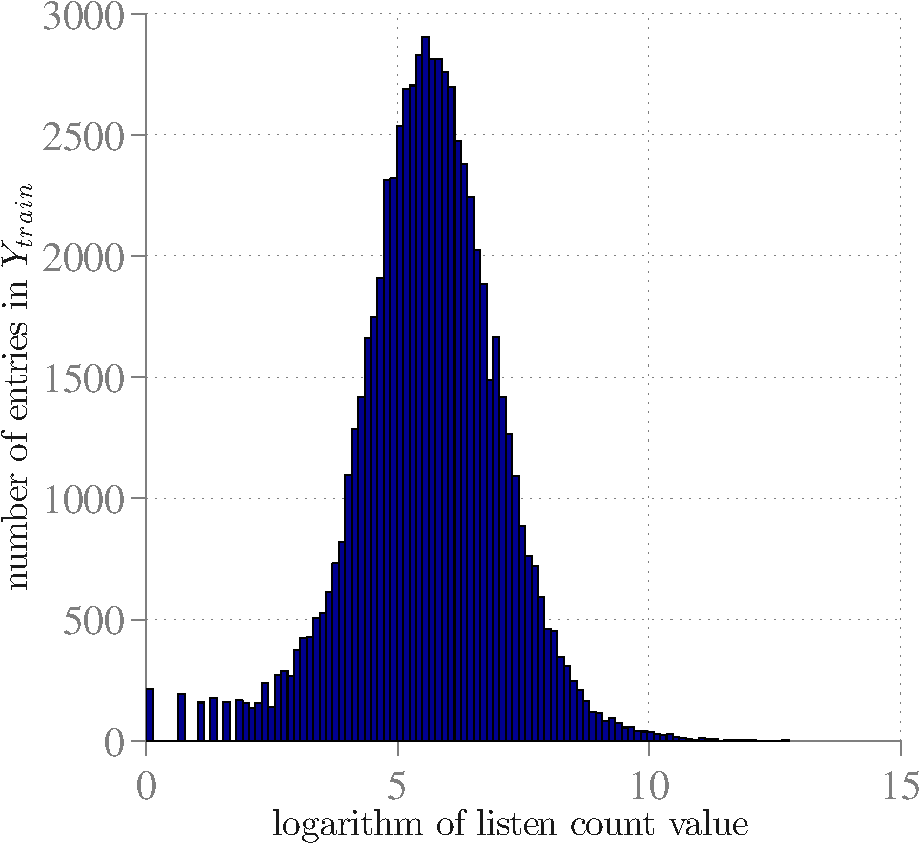
\includegraphics[width=2.5in]{../figures/log_listen_counts-crop.pdf} \label{fig:logListenCounts}}

\caption{Analysis of whole set of listen counts}
\end{figure}
As most of our models assume data is Gaussian or at least symmetric and our cost function assumes first taking logarithm of predicted listen count, we decided to apply log transformation and later set mean to $0$ and standard deviation to $1$.\footnote{We actually tested our models both on transformed and nontransformed data and got bigger errors on nontransformed data for all models} To avoid problems with null values of the matrices, we added $10^{-10}$ to any previously non-zero element. This should not change our predictions, as added value is very small (corresponding to much less then $1$ listen count even for big listen counts) and at the same time this operation is (empirically) reversible. We applied these transformations once, before any model training. All the reported errors will be mean squared errors on the transformed data.
\section{Cross-validation and test data analysis}
To evaluate different methods, we estimated our test error based on results of cross-validation. We used $5$ folds, as number of entries in the $Y_{test\_weak}$ data is around $20\%$ of those in the train matrix, so we expected to estimate test error accuarately this way.

In each fold, there is $20\%$ of the non-zero entries from the training matrix, sampled randomly. Initially, we thought about taking into test data only artists/users pairs, such that this user and artist have have more than a few (e.g. $3$) entries in the train matrix, as we expected our test data to be generated in a similiar manner (it is hard to predict anything about the user or artist we have no train data about). After drawing a figure: \ref{fig:listenersTest}, which represents number of such entries in test matrix (that corresponds to underrepresented in train matrix artists), we abandoned this idea, as most of the queries we will have to answer will be about the artists that have low ($\le 3$) number of listeners in the train dataset.

\begin{figure}[!h]
\center
\subfigure[Numbers of artists with various number of (train) listeners. We see that most of the artists have only $1$ or $2$ listeners.] {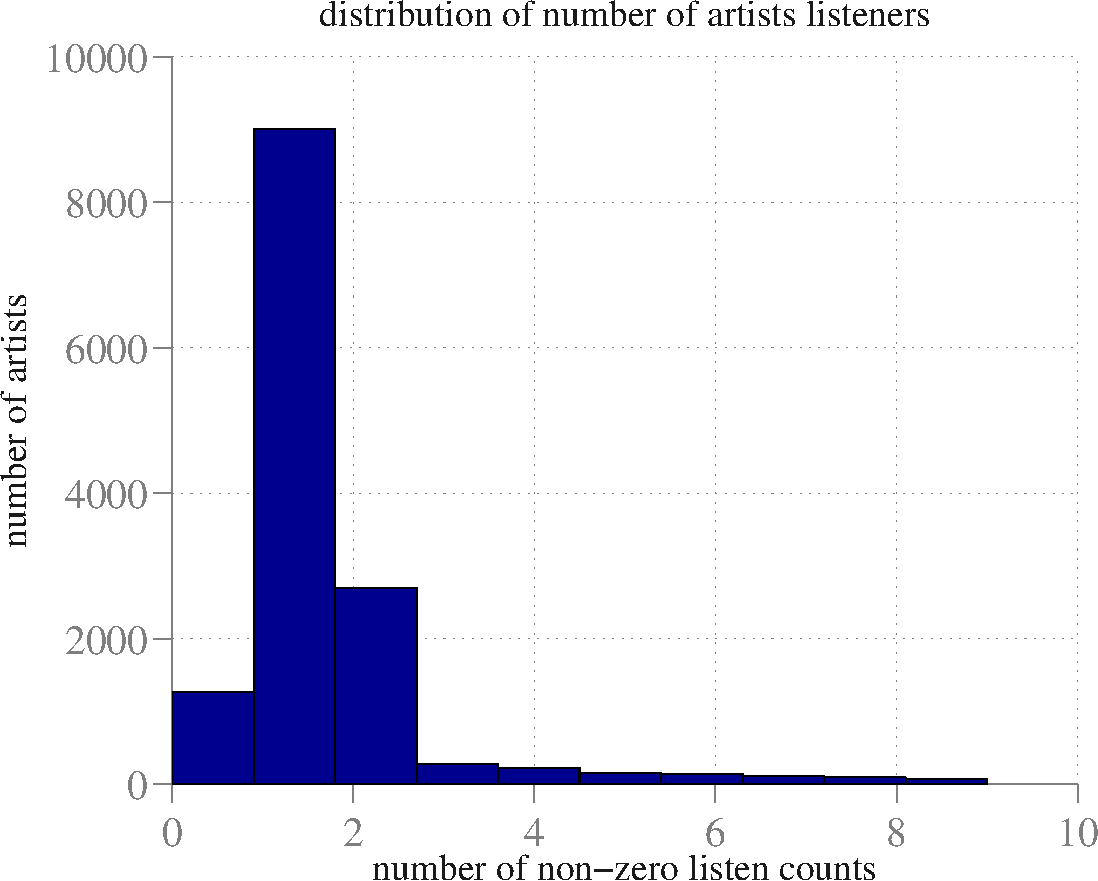
\includegraphics[width=2.5in]{../figures/artist_listeners_count-crop.pdf}}
\label{fig:artistListeners}
\subfigure[Number of entries ($Y$) in $Ytest_{weak\_pairs}$, such that a corresponding artist in the $Ytrain$ has given number of listeners ($X$). We see that for most of the test entries, we have very little data about the artist in the train dataset.]{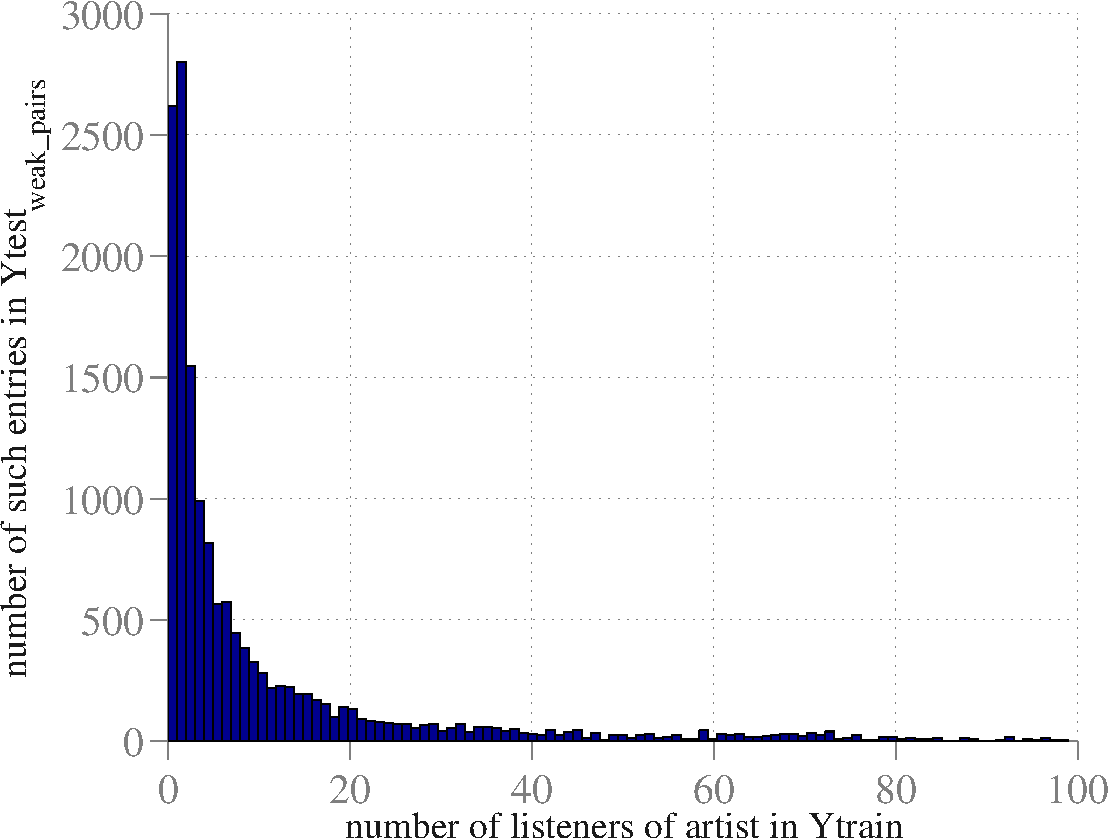
\includegraphics[width=2.5in]{../figures/listeners_number_test-crop.pdf} \label{fig:listenersTest}}
\hfill
\caption{Distribution of number of listeners of artists in the train and test datasets.}
\end{figure}

We did a similar analysis for users, and it showed that almost all users ($1762$ out of $1774$) are represented in $Ytest_{weak\_pairs}$. The distribution of number of artists each user listens to is Gaussian with mean around $40$. There is very little ($8$) entries in $Ytrain$ that corresponds to users that have listened to $< 5$ artists.

This information also justifies our later observation that there is more signal in the user row of the train matrix than in the artist column.

\section{Mean prediction} \label{meanPred}
First, very simple model we trained was to predict for each (user, artist) the average listen count of the artist. If there wasn't any listen counts for this artist in the train matrix, we predicted mean of the user, and if there were no such entries either, we predicted $0$ (which is our mean of all entries in train dataset after normalization).

We run this method with $10$ different seeds on $5$-fold cross-validation and got $MSE=1.0082$. %2.0741 without normalization
We used this result for checking other methods.

This method is implemented in file \texttt{estimateMeanPrediction.m}\footnote{As a requirement of our course project we had to provide both the code we wrote and our predictions.}

\section{Slope one algorithm}
We also implemented an easy collaborative filtering algorithm called slope one. It is described in \cite{slope} and implemented in file \texttt{estimateSlopeOne.m}. As running this algorithm as explained on the page would require $O(n^2)$ memory, where $n$ is the number of artists, we run it on the transposed matrix. Anyway, this took a lot of time to compute on the whole matrix, and gave $MSE=0.7048$.%1.4038 without normalization

\section{Alternating least-squares}
Other method, suggested by the course teacher, was Alternating least-squares (ALS, \cite{als}). We tried running it both with weighted-$\lambda$-regularization and without it - it turned out that weighting actually helps a bit (it decreased MSE error by about $0.2$). Our code can be found in file \texttt{estimateALS.m}.

As we discovered that our method sometimes predicts too big listen counts without particular reason, we decided to always return prediction that is not bigger then the biggest value in a given row and column in the train matrix.

 To choose the appropriate regularization term, we calculated $100$ random entries from reconstruction matrix (i.e. $U' * A$, where $A$ and $U$ are the two factor matrices) after two last iterations of the algorithm. We recognize our method as converging with right regularization if the average difference between corresponding entries was $< 10^{-3}$, which corresponds to difference of at most few listen counts.

To find the best value of hidden variables, i.e. a common dimension of matrices $A$ and $U$ we used grid search with cross-validation. As shown on the figure \ref{fig:alsHidden}, we first ran more grained search, and then tried some values near the best found in the first step.

After setting the number of hidden variables to $42$ we got an $MSE=0.8324$. We thought that we could improve this result by clustering the artists by the number of corresponding entries in the train error. We expected that artists that have a lot of listeners are generally more popular and that our predictions will be too small for them (because we will be averaging with less popular artists) and vice versa. After plotting the graph \ref{fig:alsErrorDist} we abandoned this idea, as on the picture we see that ratio of too big and too small predictions does not change noticeably for different kinds of artists.

\begin{figure}[!h]
\center
\subfigure[Cross-validation error for different number of hidden variables using ALS.]{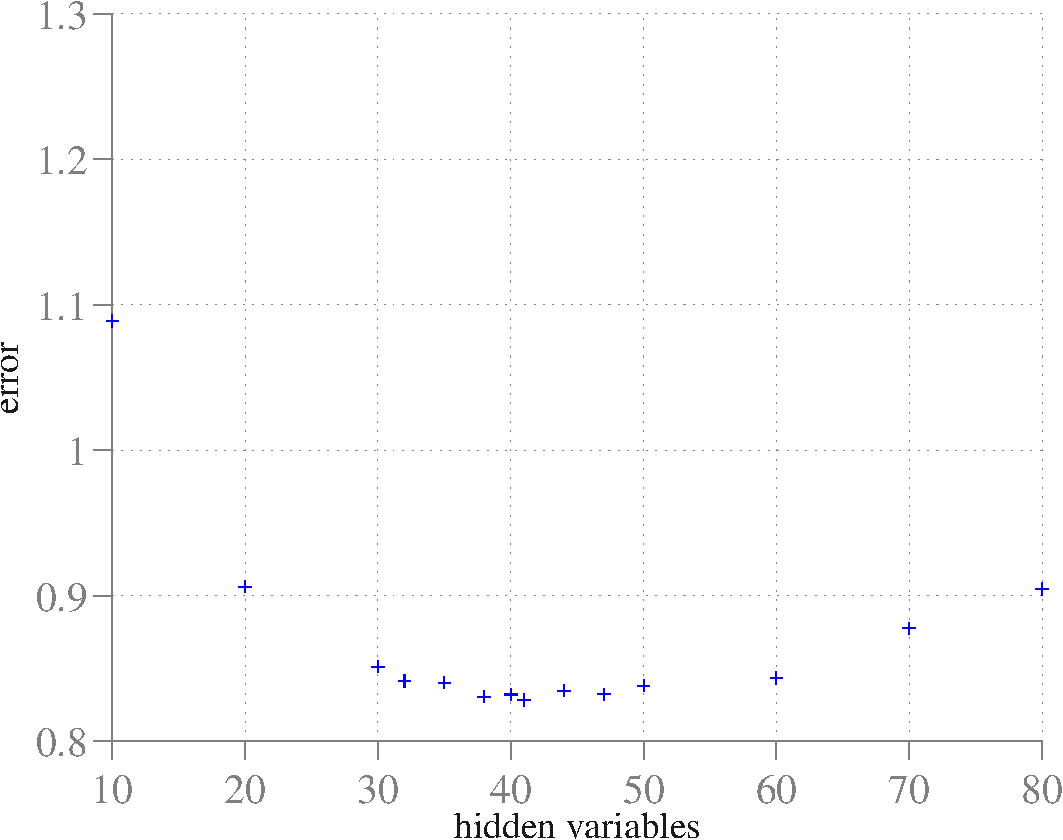
\includegraphics[width=2.5in]{../figures/als-hidden-error-crop.pdf} \label{fig:alsHidden}}
\subfigure[Error distribution in predicting listen counts of different artists.]{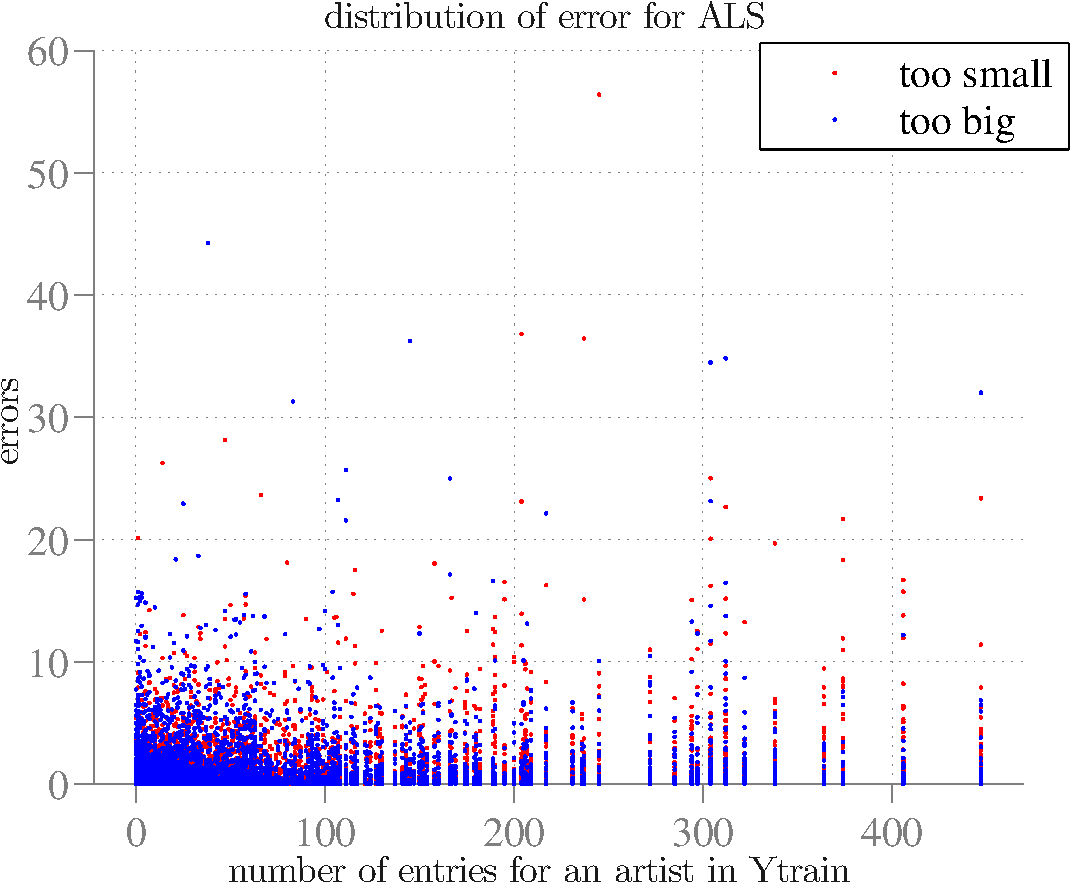
\includegraphics[width=2.5in]{../figures/als-error-dist-crop.pdf} \label{fig:alsErrorDist}}
\caption{Analysis of ALS method.}
\end{figure}

\section{K-nearest neighbours}
When we have computed $A$ and $U$ matrix factors of non-zero elements of $Ytrain$, we can treat them as the features of the artists and a matrix of users' preferences to those features. The concept is well explained in the video: \cite{cfng}. We took this approach and implemented (in \texttt{estimateKNN.m}) a method like this:
\begin{enumerate}
\item calculate $A$, $U$ - features of artists and users - using ALS
\item for each (user, artist) pair to predict, take a look at features of every other artist this user listened and every other user that listened to this artist
\item choose $K$ of those, which are nearest (in $l_1$ norm (we also tried $l_2$))) to the artist row in $A$ or, respectively, user row in $U$
\item return mean of the $K$ listen counts, which corresponds to those $K$ vectors
\end{enumerate}

To choose value of $K$ we ran cross-validation. As the training was taking some time, we decided to choose it based on results on a subset of $Ytrain$. We chose randomly $100$ users and $4000$ artists and observed lowest test error for $K=8$. After choosing the parameters we ran it on the whole matrix and received test error $MSE=0.4180$.
\begin{figure}[!h]
\center
\subfigure[Cross-validation error for different number of neighbours in KNN.]{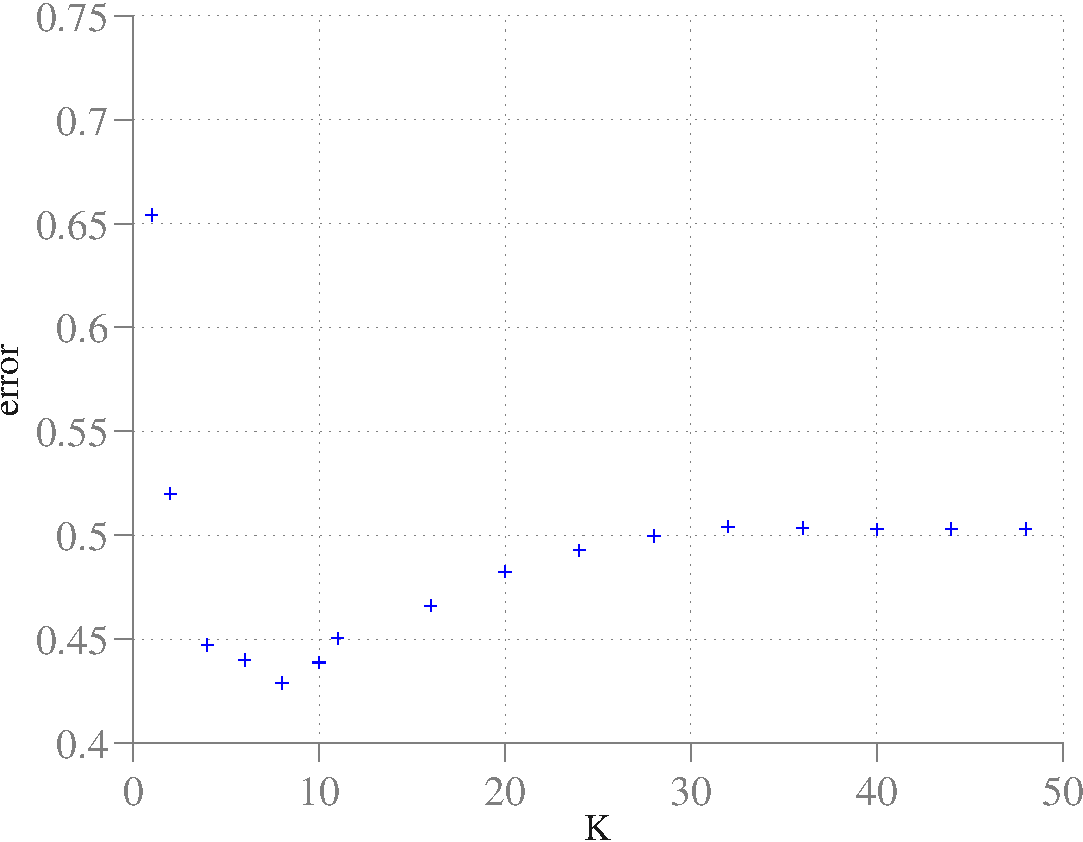
\includegraphics[width=2.5in]{../figures/knn-error-crop.pdf} \label{fig:knn}}
\subfigure[Error distribution in predicting listen counts of different artists.]{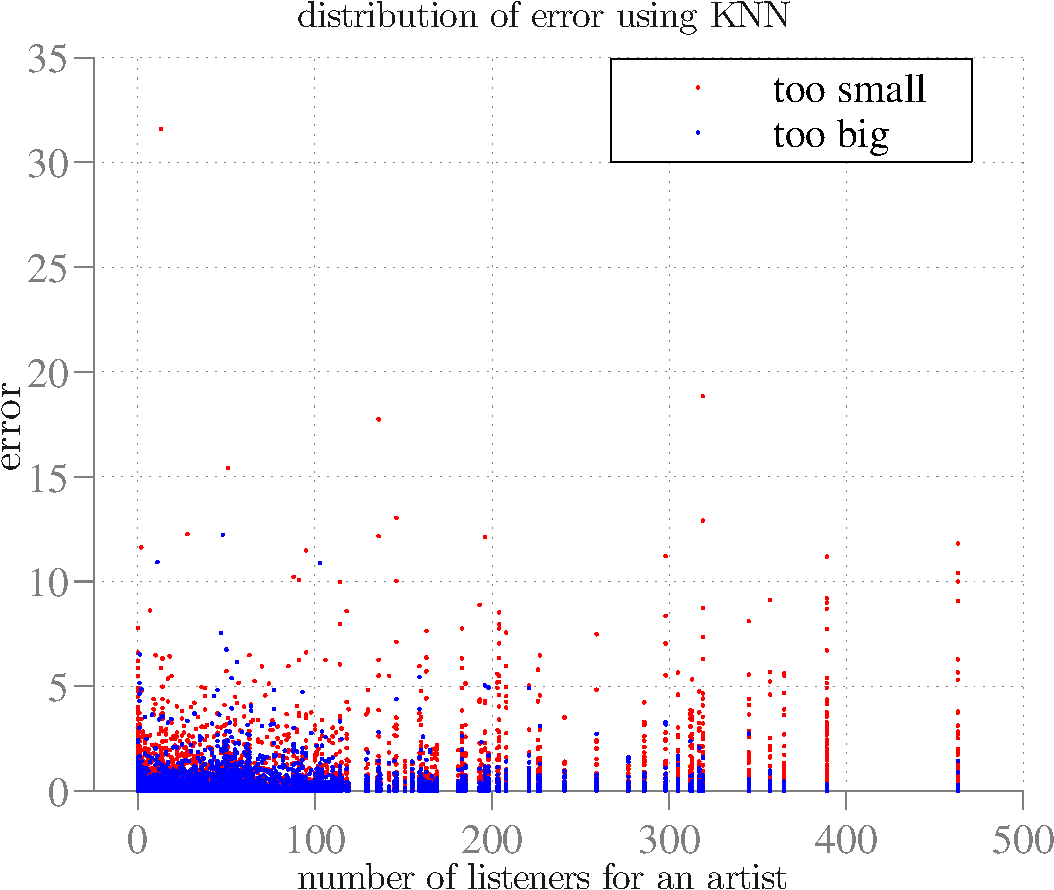
\includegraphics[width=2.5in]{../figures/knn-err-dist-crop.pdf} \label{fig:knnErrorDist}}
\caption{Analysis of KNN method.}
\end{figure}

\section{User-mean prediction}
After trying all those methods we came back to the mean prediction and tried to run it on transposed matrix (it corresponds to predicting the mean of each user listen counts). It turned out that this method works better than any previous one, giving $MSE=0.3673$. It actually makes sense, considering figure \ref{fig:artistListeners} - there is very little data for most of the artists, and we have this data about the users. This also explains why KNN works best among other methods - it takes into account user data more than other methods. We used this very simple method to give predictions for our weak dataset.

\section{Strong prediction}
For the strong prediction problem, where we don't know any data for the user except for his friends in a social network, we tried $3$ algorithms:
\begin{itemize}
\item artist-mean prediction, which is already described in section \ref{meanPred}. It gave $MSE=1.0611$.
\item to predict mean of the social network neighbours of the user. Its error was: $1.1213$. This method is implemented in file \texttt{estimateNeighbourMean.m}.
\item estimation similar to KNN algorithm: First find $A$ and $U$ decomposition using ALS, and then calculate $U2$: mean of $U$ rows corresponding to the neighbours of given user. Then, we predict (user, artist) entry as $U2 * A(artist)$ - this basically estimates user's preference row in $U$ as its neighbours' rows mean and then returns same prediction as with ALS. This method achieved $MSE$ of $1.2767$. This method is implemented in the file \texttt{estimateALSweak.m}.
\end{itemize}

As again it turned out that the best method was the simplest one, we used it to make our test predicions.

\begingroup
\renewcommand{\cleardoublepage}{}
\renewcommand{\clearpage}{}
\begin{thebibliography}{9}

\bibitem{mse}
  \url{http://en.wikipedia.org/wiki/Mean_squared_error}
\bibitem{slope}
  \url{http://en.wikipedia.org/wiki/Slope_One}
\bibitem{als}
  \url{http://www.hpl.hp.com/personal/Robert_Schreiber/papers/2008\%20AAIM\%20Netflix/netflix_aaim08\%28submitted\%29.pdf}
\bibitem{cfng}
   A. Ng online machine learning course,
   video about collaborative filtering\\
  \url{https://class.coursera.org/ml-005/lecture/100}
\bibitem{libsvm}  
Chang, Chih-Chung and Lin, Chih-Jen,
 LIBSVM: A library for support vector machines,
 
 Code available at \url{http://www.csie.ntu.edu.tw/~cjlin/libsvm}
\bibitem{piotr}
Piotr's toolbox
\url{http://vision.ucsd.edu/~pdollar/toolbox/doc/index.html}
\bibitem{rf}
\url{https://code.google.com/p/randomforest-matlab/}
\bibitem{fscore}
Yi-Wei Chen and Chih-Jen Lin,
Combining SVMs with Various Feature Selection Strategies
\url{http://www.csie.ntu.edu.tw/~cjlin/papers/features.pdf}
\bibitem{fselection}
\url{http://www.csie.ntu.edu.tw/~cjlin/libsvmtools/#feature_selection_tool}
\bibitem{hog}
\url{http://en.wikipedia.org/wiki/Histogram_of_oriented_gradients}
\bibitem{deep}
\url{https://github.com/rasmusbergpalm/DeepLearnToolbox}
\end{thebibliography}
\endgroup
\end{document}
